\documentclass[english,floatsintext,man]{apa6}

\usepackage{amssymb,amsmath}
\usepackage{ifxetex,ifluatex}
\usepackage{fixltx2e} % provides \textsubscript
\ifnum 0\ifxetex 1\fi\ifluatex 1\fi=0 % if pdftex
  \usepackage[T1]{fontenc}
  \usepackage[utf8]{inputenc}
\else % if luatex or xelatex
  \ifxetex
    \usepackage{mathspec}
    \usepackage{xltxtra,xunicode}
  \else
    \usepackage{fontspec}
  \fi
  \defaultfontfeatures{Mapping=tex-text,Scale=MatchLowercase}
  \newcommand{\euro}{€}
\fi
% use upquote if available, for straight quotes in verbatim environments
\IfFileExists{upquote.sty}{\usepackage{upquote}}{}
% use microtype if available
\IfFileExists{microtype.sty}{\usepackage{microtype}}{}

% Table formatting
\usepackage{longtable, booktabs}
\usepackage{lscape}
% \usepackage[counterclockwise]{rotating}   % Landscape page setup for large tables
\usepackage{multirow}		% Table styling
\usepackage{tabularx}		% Control Column width
\usepackage[flushleft]{threeparttable}	% Allows for three part tables with a specified notes section
\usepackage{threeparttablex}            % Lets threeparttable work with longtable

% Create new environments so endfloat can handle them
% \newenvironment{ltable}
%   {\begin{landscape}\begin{center}\begin{threeparttable}}
%   {\end{threeparttable}\end{center}\end{landscape}}

\newenvironment{lltable}
  {\begin{landscape}\begin{center}\begin{ThreePartTable}}
  {\end{ThreePartTable}\end{center}\end{landscape}}




% The following enables adjusting longtable caption width to table width
% Solution found at http://golatex.de/longtable-mit-caption-so-breit-wie-die-tabelle-t15767.html
\makeatletter
\newcommand\LastLTentrywidth{1em}
\newlength\longtablewidth
\setlength{\longtablewidth}{1in}
\newcommand\getlongtablewidth{%
 \begingroup
  \ifcsname LT@\roman{LT@tables}\endcsname
  \global\longtablewidth=0pt
  \renewcommand\LT@entry[2]{\global\advance\longtablewidth by ##2\relax\gdef\LastLTentrywidth{##2}}%
  \@nameuse{LT@\roman{LT@tables}}%
  \fi
\endgroup}


  \usepackage{graphicx}
  \makeatletter
  \def\maxwidth{\ifdim\Gin@nat@width>\linewidth\linewidth\else\Gin@nat@width\fi}
  \def\maxheight{\ifdim\Gin@nat@height>\textheight\textheight\else\Gin@nat@height\fi}
  \makeatother
  % Scale images if necessary, so that they will not overflow the page
  % margins by default, and it is still possible to overwrite the defaults
  % using explicit options in \includegraphics[width, height, ...]{}
  \setkeys{Gin}{width=\maxwidth,height=\maxheight,keepaspectratio}
\ifxetex
  \usepackage[setpagesize=false, % page size defined by xetex
              unicode=false, % unicode breaks when used with xetex
              xetex]{hyperref}
\else
  \usepackage[unicode=true]{hyperref}
\fi
\hypersetup{breaklinks=true,
            pdfauthor={},
            pdftitle={Common or Distinct Attention Mechanisms for Contrast and Assimilation?},
            colorlinks=true,
            citecolor=blue,
            urlcolor=blue,
            linkcolor=black,
            pdfborder={0 0 0}}
\urlstyle{same}  % don't use monospace font for urls

\setlength{\parindent}{0pt}
%\setlength{\parskip}{0pt plus 0pt minus 0pt}

\setlength{\emergencystretch}{3em}  % prevent overfull lines

\ifxetex
  \usepackage{polyglossia}
  \setmainlanguage{}
\else
  \usepackage[english]{babel}
\fi

% Manuscript styling
\captionsetup{font=singlespacing,justification=justified}
\usepackage{csquotes}
\usepackage{upgreek}



\usepackage{tikz} % Variable definition to generate author note

% fix for \tightlist problem in pandoc 1.14
\providecommand{\tightlist}{%
  \setlength{\itemsep}{0pt}\setlength{\parskip}{0pt}}

% Essential manuscript parts
  \title{Common or Distinct Attention Mechanisms for Contrast and Assimilation?}

  \shorttitle{Contrast and Assimilation}


  \author{Hope K. Snyder\textsuperscript{1}, Sean M. Rafferty\textsuperscript{1}, Julia M. Haaf\textsuperscript{1}, \& Jeffery N. Rouder\textsuperscript{2,1}}

  % \def\affdep{{"", "", "", ""}}%
  % \def\affcity{{"", "", "", ""}}%

  \affiliation{
    \vspace{0.5cm}
          \textsuperscript{1} University of Missouri\\
          \textsuperscript{2} University of California, Irvine  }

  \authornote{
    This document was written in R-Markdown with code for data analysis
    integrated into the text. The Markdown script is open and freely
    available at
    \url{https://github.com/PerceptionAndCognitionLab/ctx-flanker/tree/public/papers/current}.
    The data were \emph{born open} (Rouder, 2016) and are freely available
    at
    \url{https://github.com/PerceptionCognitionLab/data1/tree/master/ctxIndDif/flankerMorph4}
    
    Correspondence concerning this article should be addressed to Hope K.
    Snyder, 205 McAlester Hall, University of Missouri, Columbia, MO 65211.
    E-mail:
    \href{mailto:hks7w2@mail.missouri.edu}{\nolinkurl{hks7w2@mail.missouri.edu}}
  }


  \abstract{The ability to inhibit distractors while focusing on specific targets is
crucial. In most tasks, like Stroop or priming, the to-be-ignored
distractors affect the response to be more like the distractors. We call
that assimilation. Yet, in some tasks, contrast tasks, the opposite
holds. Contrast and assimilation are opposing behavioral effects, but
they both occur when to-be-ignored information affects judgments. We ask
here whether inhibition across contrastive and assimilative tasks is
common or distinct. Assimilation and contrast are often thought to have
different underlying psychological mechanisms, and we use a
correlational analysis with hierarchical Bayesian models as a test of
this hypothesis. We designed tasks with large assimilation or contrast
effects. The stimuli are morphed letters, and whether there is contrast
or assimilation depends on whether the surround is a letter field
(contrast) or a word field (assimilation). Critically, a positive
correlation was found - individuals who better inhibited
contrast-inducing contexts also better inhibited assimilation-inducing
contexts. These results indicate inhibition is common, at least in part,
across contrast and assimilation tasks.}
  \keywords{Inhibition, Selective Attention, Contrast Effects, Assimilation Effects \\

    
  }





\usepackage{amsthm}
\newtheorem{theorem}{Theorem}
\newtheorem{lemma}{Lemma}
\theoremstyle{definition}
\newtheorem{definition}{Definition}
\newtheorem{corollary}{Corollary}
\newtheorem{proposition}{Proposition}
\theoremstyle{definition}
\newtheorem{example}{Example}
\theoremstyle{definition}
\newtheorem{exercise}{Exercise}
\theoremstyle{remark}
\newtheorem*{remark}{Remark}
\newtheorem*{solution}{Solution}
\begin{document}

\maketitle

\setcounter{secnumdepth}{0}



The concepts of \emph{spatial selective attention} and \emph{response
inhibition} have been topical in the psychological literature since at
least Helmholtz (1867) and James (1890). The ability to inhibit some
elements in the environment while focusing on other target elements is
crucial to proper functioning (e.g., Broadbent, 1958; Cowan, 1995).
Failures to properly inhibit responses to inappropriate elements in the
environment are used to describe and understand pathological development
(Barkley, 1997; Hasher \& Zacks, 1988). Inhibition is usually treated as
a fairly unified or homogenous concept. It may be measured in tasks
where the goal is to select or identify target items in the presence of
to-be-ignored distractors. We provide a novel and, in our opinion, an
exceedingly strong test of whether spatial inhibition is a unified
phenomenon.

In many spatial interference tasks, such as Eriksen interference (B. A.
Eriksen \& Eriksen, 1974), the effect is usually in a specific direction
that we term \emph{assimilation}. Assimilation is displayed in Figure
\ref{fig:past}A where the goal is to identify the center letter as
either an \enquote{A} or an \enquote{H.} People are more likely to
misidentify the target \emph{H} as an \enquote{A} when surrounded by
\emph{A}'s than surrounded by \emph{H}'s. Because they are making
responses seemingly driven by the identity of the flankers rather than
the target, we say their inhibition failure leads to an
\emph{assimilation} of the background.

Assimilation, however, is not the only outcome. Rouder and King (2003)
used a modified version of the flanker task and found the opposite
effects, which are called here \emph{contrast} effects. Rather than use
well-formed letters, Rouder and King's targets were morphed letters
between \emph{A} and \emph{H} (see Figure \ref{fig:past}B). Perhaps
surprisingly, morphs surrounded by \emph{H}'s were \emph{less likely} to
be identified as \enquote{H} than morphs surrounded by \emph{A}'s. This
effect is exactly opposite because inhibition failures lead to a
response that is in contrast to the background.

\begin{figure}[htbp]
\centering
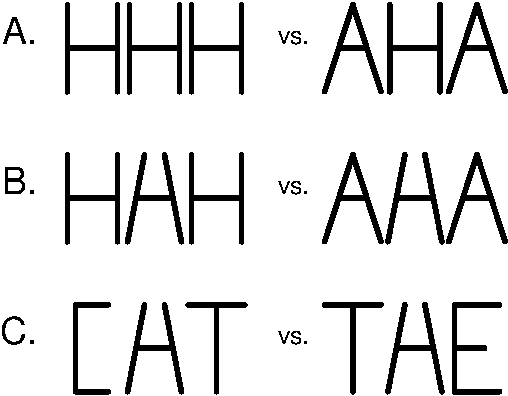
\includegraphics{paper_files/figure-latex/past-1.pdf}
\caption{\label{fig:past}Three flanker paradigms. The participants' task is
to identify the center letter as either an A or an H. \textbf{A.}
Conventional Eriksen \& Eriksen (1974) flanker paradigm results in
assimilation. \textbf{B.} Modified paradigm with morph-letter targets
results in contrast (Rouder \& King, 2003). \textbf{C.} Word contexts
result in assimilation (Neisser, 1967).}
\end{figure}

The presence of two different attention effects, assimilation and
contrast, provides a fruitful window for examining the unity of
inhibition. Both contrast and assimilation here reflect a failure to
completely inhibit the background, but they lead to opposite behavioral
patterns. The question then is whether the inhibition processes are the
same in both tasks. We address this question by studying the correlation
of inhibition abilities across people. Are people who are good at
ignoring the surrounding information in a standard flanker task that
promote assimilation also good at ignoring the surrounding information
in a modified flanker task that promotes contrast?

Correlation studies across attention tasks are certainly popular in
cognition. Indeed, far more expansive studies than ours which provide
for far more correlations across tasks have been performed (Barrett,
Tugade, \& Engle, 2004; Miyake et al., 2000). To the best of our
knowledge, these studies use assimilative inhibition tasks such as the
flanker interference with well-formed letters and anti-saccade tasks. In
fact, we are unaware of any individual-differences studies that use
contrast tasks. Here, we compare the correlations among people with
contrast and assimilation. Such a a positive correlation, if found,
provides stronger evidence for a unified concept than just assimilation
tasks because the correlation relates behaviorally opposing effects.

The current literature on whether there should be common inhibition
mechanisms across assimilation and contrast tasks is mixed. Support for
the common-mechanism view is as follows: Most proposed behavioral and
neural mechanisms of selective attention rely on a narrowing of
receptive fields. This narrowing process occurs whether the
to-be-excluded information is contrastive or assimilative (e.g., Cowan,
1995; Desimone \& Duncan, 1995; Eriksen \& Schultz, 1979; Hedden \&
Gabrieli, 2010). Behavioral evidence comes from Miyake et al. (2000) who
studied individual differences. When variability across a range of
executive-function tasks is decomposed, one recovered latent factor is a
unified concept of inhibition. Yet, there are strong arguments that
contrast and assimilation are not the same process. Most theories of
contrast rely on a center-surround organization of low-level, perceptual
receptive field structures (Palmer, 1999). Most theories of assimilation
flanker effects, however, are failures of response inhibition, which is
conceptualized as a higher-level, top down process (B. A. Eriksen \&
Eriksen, 1974). Behavioral evidence for distinct processes comes from
Rouder and King (2003) whose design is a bit complicated. These
researchers associated the letters \emph{c} and \emph{A} with one
response, denoted \(R_1\), and \emph{e} and \emph{H} with another,
denoted \(R_2\). When well-formed letters were the target, assimilation
to the response assignment of the background was observed. For
well-formed \emph{A} letters, backgrounds of \emph{c} resulted in higher
proportion of \(R_1\) response than did backgrounds of \emph{e}. When
morphed letters were targets, the effect varied. If morphs between
\emph{A} and \emph{H} were surrounded by either \emph{A} or \emph{H},
the effect was contrastive. Yet, if these same morphs were surrounded by
\emph{c} or \emph{e}, the effect was assimilative. Rouder and King
(2003) interpreted the assimilative effect to be at the response level
and the contrastive effect to be at a perceptual level.

We employ better stimulus control than Rouder and King (2003). We sought
targets and backgrounds such that whether there was contrast or
assimilation was a function of the background rather than the target.
Our targets were morphed letters like those in Figure \ref{fig:past}B.
Our backgrounds came in two types, either a letter context such as in
Figure \ref{fig:past}B or a word context such as in \ref{fig:past}C. For
the letter context, we expect large contrast effects as was observed by
Rouder and King (2003). The rationale for the word context comes from
Neisser (1967). We expect that a morph between \emph{A} and \emph{H}
will be judged more \enquote{A} like in \emph{C\_T} context than
\emph{T\_E} context. This effect is assimilative, and it has been
repeatedly demonstrated that there is an assimilative effect of word
contexts for both visually and orally presented letters (Baron \&
Thurston, 1973; Reicher, 1969). As an aside, this assimilation effect
has been a motivating phenomenon in the development of connectionist
models (e.g., Carpenter \& Grossberg, 1987; Rumelhart \& McClelland,
1982) where word nodes feed positive activation to corresponding letter
nodes.

In the following experiment, each participant identified several
\emph{A}-to-\emph{H} morphs (see the top row of Figure
\ref{fig:stimulus}). These target morphs were embedded within four
background contexts (see the bottom row of Figure \ref{fig:stimulus}).
By comparing performance in the \emph{A}-letter and \emph{H}-letter
contexts, we assess each participant's ability to inhibit contrastive
information. By comparing performance in the \emph{C\_T}-word and
\emph{T\_E}-word contexts, we assess each participant's ability to
inhibit assimilative information. Note that for each target, there are
assimilative and contrastive background contexts such that the critical
comparisons may be made across backgrounds. To assess the question of
whether inhibition across contrastive and assimilative contexts is
common or distinct, we assess the correlation across individuals of
their inhibition within the two context types.

\section{Method}\label{method}

\subsection{Sample Size Consideration}\label{sample-size-consideration}

The following experiment is a massively repeated within-subjects design.
Each participant observes 960 trials, a number that was as large as
possible within an hour time frame. The critical question is how many
participants to use, and the key consideration is whether the main
source of variability is within-trial noise or across-participant noise.
There is little guidance in the literature, and as a consequence we used
a sequential approach where the critical Bayes factor, to be discussed
subsequently, reached a ratio of 5-to-1 (Rouder, 2014). In reality, we
ran out even after reaching this goal to provide opportunities for
participants to take part. We ended with 93 usable participants who made
65,541 usable responses, and our Bayes factor was 25-to-1. Although our
protocol was not preregistered and did not follow a set sequential plan,
we exercised good judgment. Readers wishing the check can do so. All of
our data were made publicly available as they were collected and may be
found at
\url{https://github.com/PerceptionCognitionLab/data1/tree/master/ctxIndDif/flankerMorph4}.
This mode of data collection is called Born Open Data (Rouder, 2016) and
readers can see the effects of stopping at any point.

\subsection{Participants}\label{participants}

Ninety-nine undergraduates from the University of Missouri served as
participants as part of an introductory course requirement. Data from
two participants were discarded due to a computer error and data from an
additional four were discarded because twenty or more of their responses
were shorter than a criterial 200 ms in duration. The data from the
remaining \(93\) participants were used in analysis.

\subsection{Design}\label{design}

The experiment was a \(5\times 2 \times 2\) within-subject factorial
design. The first factor was the target, and it was manipulated through
5 levels from the letter \emph{H} through the morphs to the letter
\emph{A}. The second factor was the context type, and the background was
either a letter or a word. The final variable was context direction, a
context that promotes \enquote{A} or \enquote{H} responses. We coded the
\emph{H} background and the \emph{C\_T} background as promoting
\enquote{A} responses based on prior literature. This coding does not
determine the direction of results; it simply provides a clear language
for discussing them.

\begin{figure}[htbp]
\centering
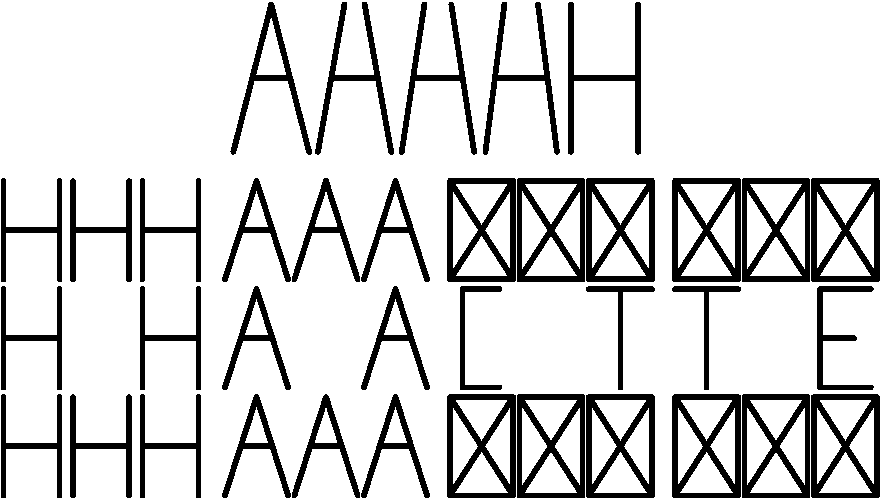
\includegraphics{paper_files/figure-latex/stimulus-1.pdf}
\caption{\label{fig:stimulus}Stimuli. \textbf{Top} Five targets.
\textbf{Bottom} Four contexts. The stimulus on a trial consisted of one
of the four targets placed into the blank center location of the
background context.}
\end{figure}

\subsection{Material}\label{material}

The stimuli are shown in Figure \ref{fig:stimulus}. All targets appear
in each of the four contexts, though the rates are not equal. To
emphasize the morphs, the three central targets in Figure
\ref{fig:stimulus} were each twice as likely to appear than each
well-formed letter.

\subsection{Procedure}\label{procedure}

Participants were presented with the stimuli and asked to judge whether
the center letter was more similar to an \enquote{A} or an \enquote{H}
by pressing the corresponding keys on a standard keyboard. Participants
were explicitly instructed to ignore the background context and base
their responses on the central target alone.

An experimental trial proceeded as follows: The screen was blank during
a 1.5 sec foreperiod. We warned participants that a target was about to
appear as follows. Two brief tones were presented 500 ms and 250 ms
before the stimulus. These tones allowed participants to precisely time
the stimulus. Next, the stimulus was presented for 100 ms, and
thereafter, was replaced by a blank screen. This blank screen remained
until participant pressed either the \enquote{A} or \enquote{H} key to
indicate their judgment about the target. The response marked the end of
the current trial and the beginning of the next one. Responses and the
time taken to respond was recorded. A block consisted of 96 trials and
the experimental session consisted of 10 blocks for a total of 960
trials. Participants were encouraged to take breaks between blocks. No
feedback was given about participant responses during the course of the
experimental session.

All experimental sessions were conducted on MacMini computers running
the operating system MacOSX 10.6.2 with Octave version 3.2.3. This
experimental procedure was approved by the Institutional Review Board at
the University of Missouri.

\section{Results}\label{results}

Data were cleaned by discarding responses with latencies less than 200
ms and greater than 2 sec.~These discards comprised about 1\% of the
total. Additionally, the first twenty trials of the session were
considered practice and excluded. These criteria were chosen before data
collection.

Figures \ref{fig:avcfigures}A and B show the proportion of \enquote{H}
responses as a function of target and context. As expected, the curves
start low for \emph{A} and \emph{A}-like stimuli and increase as the
targets become more \emph{H}-like. Figure \ref{fig:avcfigures}A displays
the results for the letter contexts (\emph{A}-letter and
\emph{H}-letter) and Figure \ref{fig:avcfigures}B displays results for
the word contexts (\emph{C\_T}-word and \emph{T\_E}-word). Solid and
dashed lines differentiate in each graph differentiates the contexts in
each graph from one another. A contrast effect may be seen for letter
contexts. Here, the \emph{A}-letter context promoted higher proportions
of \enquote{H} responses than the \emph{H}-letter context did. The
opposed effect---assimilation---may be seen for the word contexts. The
context \emph{T\_E} promoted higher proportions of \enquote{H} responses
than the \emph{C\_T} context did.

\begin{figure}[htbp]
\centering
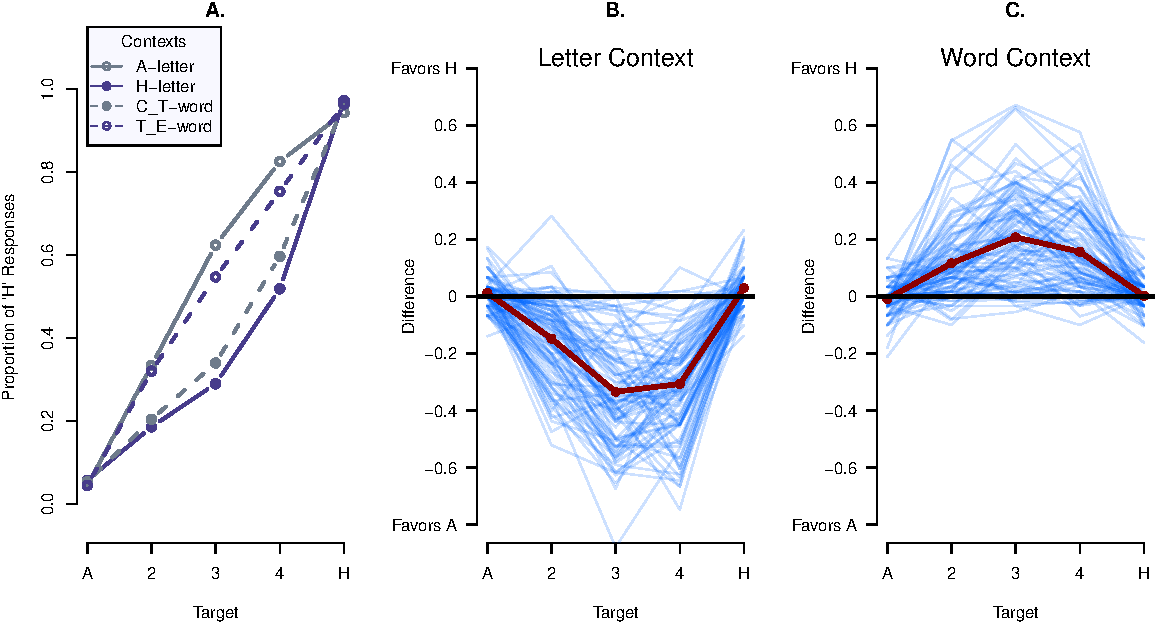
\includegraphics{paper_files/figure-latex/avcfigures-1.pdf}
\caption{\label{fig:avcfigures}Empirical Results. \textbf{A.} Response
proportions for letter contexts. Solid and dashed lines differentiate
between A-letter and H-letter contexts. \textbf{B.} Response proportions
for word contexts. Solid and dashed lines differentiate between
C\_T-word and T\_E-word contexts. \textbf{C.} Individual effects in the
letter contexts. The negative direction denotes a robust contrast
effect. \textbf{D.} Individual effects in the word contexts. The
positive direction denotes a robust assimilation effect.}
\end{figure}

Figures \ref{fig:avcfigures}A and B show effects averaged across
individuals. Effects for each individual are shown in Panels C and D. To
observe individual effects in the letter-context condition, we
subtracted the proportion of \enquote{H} responses for the
\emph{A}-letter context from that for the \emph{H}-letter context. In
this graph, positive values indicate an assimilation effect; zero
indicates no effect of context direction; negative values indicate a
contrast effect. The following three points are noted: 1) The contrast
effects of letter contexts are robust across individuals. 2) The size of
these effects is much larger than usual. The differences in proportions
average as much as 0.34, which dwarfs the size of differences in most
experiments. 3) The degree of individual variability is also quite
large. This degree provides increased resolution in the following
correlational analysis. Figure \ref{fig:avcfigures}D shows the same plot
for the word context; it is formed by subtracting the proportion of H
responses in the \emph{C\_T}-word context from that in the
\emph{T\_E}-word context. The story about individuals is largely the
same: 1) seemingly every individual shows an assimilation effect, 2) the
effect is large, averaging as much as 0.21, and 3) there is a suitable
range of variation.

To assess the correlation among individual assimilation and contrast
effects, we developed a Bayesian hierarchical mixed model with a probit
link. The benefits of the modeling approach are two-fold: First, it
provides a principled means of combining data across the different
targets. Second, and more importantly, the hierarchical structure
provides a form of regularization used to avoid overstating the range of
individual variation (Davis-Stober, Dana, \& Rouder, 2017; Efron \&
Morris, 1977; Lehmann \& Casella, 1998). The model and corresponding
analysis are described in an online supplement at
\url{https://github.com/PerceptionAndCognitionLab/ctx-flanker/tree/public/papers/current}.
The main outputs are individual estimates of assimilation and contrast
effects and a posterior distribution of the correlation. The individual
estimates are shown in the scatter plot in Figure
\ref{fig:modelfiguresminus}A; more positive values indicate a stronger
assimilation and stronger contrast effects in the respective background
contexts.

\begin{figure}[htbp]
\centering
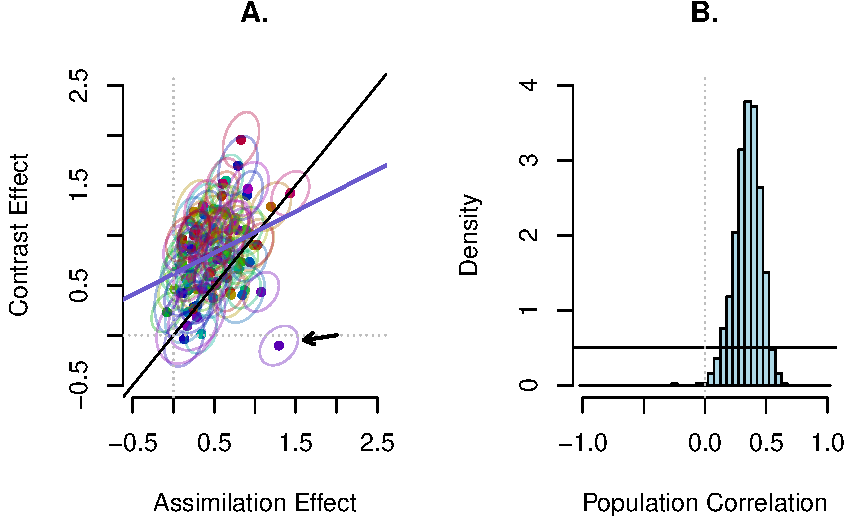
\includegraphics{paper_files/figure-latex/modelfiguresminus-1.pdf}
\caption{\label{fig:modelfiguresminus}Model Results. \textbf{A.} Each
participant's estimated assimilation effect against their estimated
contrast effect. An ellipse denotes the standard deviations of the
estimate and the blue regression line is the line of best fit.
\textbf{B.} The posterior distribution of the population correlation,
\(\rho\), between assimilation and contrast. The solid line denotes the
prior distribution.}
\end{figure}

As can be seen in Figure \ref{fig:modelfiguresminus}A, there is a fair
degree of variation across individuals as well as an overall positive
relationship. An issue, however, is the presence of an outlying point,
indicated with an arrow. This participant had the highest degree of
assimilation and the lowest degree of contrast. Performance here stands
apart from that of the other participants; if the points is included in
analysis, then it would have great leverage. We decided in a
\emph{post-hoc} manner to exclude this participant, and the following
analyses are based on this exclusion. Our results therefore pertain to
the vast majority of individuals in the main cluster.

Assimilation and contrast estimates show a positive relationship as seen
by the OLS regression line in Figure \ref{fig:modelfiguresminus}A. OLS
regression, however, is inappropriate as an inferential tool because the
estimates are correlated through the hierarchical structure. To perform
inference, we plot the prior and posterior distributions of the
population-level correlation coefficient. The prior distribution here
was chosen to be flat, placing equal plausibility on all values of the
correlation coefficient. The resulting posterior distribution is well
localized for positive values away from zero. The mean of this posterior
distribution serves as a point estimate, and it is 0.23. One way of
competitively assessing the null-correlation hypothesis vs.~the
alternative is to compute the change in plausibility at zero. The
plausibility was greatly reduced by a factor of 1. This indicates the
data are 1 times more plausible under the alternative than the null, and
this computation is the Savage-Dickey approach to Bayes factors (Dickey,
1971; Gelfand \& Smith, 1990).

To place this correlation in context, it is helpful to consider the
reliability of individual estimates. We suspected high reliability
because we had each participant perform a total of 960 trials, which is
quite numerous. We split each individual's data into odd and even
trials, and reran the Bayesian probit regression analysis separately for
the odd and even trials. Each analysis provides an estimate of each
individual's assimilation and contrast, and the assimilation estimates
in the odd trials may be correlated with the assimilation in the even
trials, and the same for the contrast estimates. The correlation among
individuals' assimilation estimates was 0.76; the correlation among
individuals' contrast estimates was 0.78. These values when extrapolated
to the full sample imply reliabilities of 0.86 and 0.87, respectively.
Hence, much of the variation in the scatter is not due to trial-by-trial
noise, but reflect true latent variation across individuals.

\section{Discussion}\label{discussion}

Our goal here was to explore whether inhibition was mediate by a common
or distinct mechanisms in assimilation and contrast contexts. On one
hand, inhibition is often conceptualized as a well-integrated concept
(e.g., Miyake et al., 2000). On the other hand, assimilation is often
thought of as a response-level cognitive process (B. A. Eriksen \&
Eriksen, 1974) whereas contrast is thought of as a low-level perceptual
process (e.g., Palmer, 1999). To explore this question, we assessed the
correlation between individuals' ability to inhibit background
assimilative information and their ability to inhibit background
contrastive information. Our approach relied on morph-letter targets.
Large assimilation effects were found when the surrounding,
to-be-ignored information could potentially be a word, replicating the
often observed top-down effect of word contexts on letter
identification. Contrast effects were found when the surrounding
contexts were letters, replicating Rouder and King (2003). The key
finding is a positive correlation across individuals. Individuals who
were better able to inhibit the contrastive effects of surrounding
letter contexts were better able to inhibit the assimilative effects of
surrounding word contexts.

The findings are surprising inasmuch as contrast and assimilation
effects are generally thought to have different loci. We think the
correlation is of interest in itself. Perhaps the most parsimonious
account is from Lachter, Forster, and Ruthruff (2004), who provide an
updated version of Broadband's classic early-attention theory
(Broadbent, 1958). Here attention acts fairly early but is imperfect and
some irrelevant information is processed. When it is, the ensuing
contrast and assimilation effects result. In this view, the common
variation across these tasks indexes the individual's raw ability to
control selective attention. Linking correlations with processing must
be done tentatively. The next step forward in this line of research is
exploring how the correlations across contrastive and assimilative tasks
interact with manipulations designed to affect spatial attention.

\paragraph{Author's Contributions}\label{authors-contributions}

H.K.S. helped conceive the project, programed the experiment, performed
the Bayesian data analysis, and contributed to the writing of the
manuscript. S. M. R. led data collection and provided initial analysis
of the data. J. M. H. contributed to the design and data analysis. J. N.
R. contributed to all aspects of the project except for data collection.
All authors take responsibility for the integrity of the data, analysis,
and interpretation.

\newpage

\section{References}\label{references}

\setlength{\parindent}{-0.5in} \setlength{\leftskip}{0.5in}

\hypertarget{refs}{}
\hypertarget{ref-Barkley:1997}{}
Barkley, R. A. (1997). Behavioral inhibition, sustained attention, and
executive functions: Constructing a unifying theory of adhd.
\emph{Psychological Bulletin}, \emph{121}(1), 65.

\hypertarget{ref-Baron:Thurston:1973}{}
Baron, J., \& Thurston, I. (1973). An analysis of the word-superiority
effect. \emph{Cognitive Psychology}, \emph{4}(2), 207--228.

\hypertarget{ref-Barrett:etal:2004}{}
Barrett, L. F., Tugade, M. M., \& Engle, R. W. (2004). Individual
differences in working memory capacity and dual-process theories of the
mind. \emph{Psychological Bulletin}, \emph{130}(4), 553--573.

\hypertarget{ref-Broadbent:1958}{}
Broadbent, D. E. (1958). \emph{Perception and communication}. New York:
Oxford University Press.

\hypertarget{ref-Carpenter:Grossberg:1987}{}
Carpenter, G. A., \& Grossberg, S. (1987). A massively parallel
architecture for a self-organizing neural pattern recognition machine.
\emph{Computer Vision, Graphics, and Image Processing}, \emph{37}(1),
54--115.

\hypertarget{ref-Cowan:1995}{}
Cowan, N. (1995). \emph{Attention and memory: An integrated framework}.
Oxford University Press.

\hypertarget{ref-Davis:etal:2017}{}
Davis-Stober, C., Dana, J., \& Rouder, J. N. (2017). When are sample
means meaningful? The role of modern estimation in psychological
science. \emph{Open Science Framework. April}, \emph{12}.

\hypertarget{ref-Desimone:Duncan:1995}{}
Desimone, R., \& Duncan, J. (1995). Neural mechanisms of selective
visual attention. \emph{Annual Review of Neuroscience}, \emph{18}(1),
193--222.

\hypertarget{ref-Dickey:1971}{}
Dickey, J. M. (1971). The weighted likelihood ratio, linear hypotheses
on normal location parameters. \emph{The Annals of Mathematical
Statistics}, \emph{42}(1), 204--223. Retrieved from
\url{http://www.jstor.org/stable/2958475}

\hypertarget{ref-Efron:Morris:1977}{}
Efron, B., \& Morris, C. (1977). Stein's paradox in statistics.
\emph{Scientific American}, \emph{236}, 119--127.

\hypertarget{ref-Eriksen:Eriksen:1974}{}
Eriksen, B. A., \& Eriksen, C. W. (1974). Effects of noise letters upon
the identification of a target letter in a nonsearch task.
\emph{Perception \& Psychophysics}, \emph{16}, 143--149.

\hypertarget{ref-Eriksen:Schultz:1979}{}
Eriksen, C. W., \& Schultz, D. (1979). Information processing in visual
search: A continuous flow conception and experimental results.
\emph{Perception \& Psychophysics}, \emph{25}, 249--263.

\hypertarget{ref-Gelfand:Smith:1990}{}
Gelfand, A., \& Smith, A. F. M. (1990). Sampling based approaches to
calculating marginal densities. \emph{Journal of the American
Statistical Association}, \emph{85}, 398--409.

\hypertarget{ref-Hasher:Zacks:1988}{}
Hasher, L., \& Zacks, R. T. (1988). Working memory, comprehension, and
aging: A review and a new view. In G. H. Bower (Ed.), \emph{The
psychology of learning and motivation: Advances in research and theory}
(Vol. 22, pp. 193--225). Academic Press.

\hypertarget{ref-Hedden:Gabrieli:2010}{}
Hedden, T., \& Gabrieli, J. D. (2010). Shared and selective neural
correlates of inhibition, facilitation, and shifting processes during
executive control. \emph{Neuroimage}, \emph{51}(1), 421--431.

\hypertarget{ref-Helmholtz:1867}{}
Helmholtz, H. von. (1867). Treatise on physiological optics vol. iii.

\hypertarget{ref-James:1890a}{}
James, W. (1890). \emph{Principles of psychology (Volume I)}. New York:
Holt. Retrieved from
\url{http://psychclassics.yorku.ca/James/Principles/index.htm}

\hypertarget{ref-Lachter:etal:2004}{}
Lachter, J., Forster, K. I., \& Ruthruff, E. (2004). Forty-five years
after broadbent (1958): Still no identification without attention.
\emph{Psychological Review}, \emph{111}(4), 880.

\hypertarget{ref-Lehmann:Casella:1998}{}
Lehmann, E. L., \& Casella, G. (1998). \emph{Theory of point estimation,
2nd edition}. New York: Springer.

\hypertarget{ref-Miyake:etal:2000}{}
Miyake, A., Friedman, N. P., Emerson, M. J., Witzki, A. H., Howerter,
A., \& Wager, T. D. (2000). The unity and diversity of executive
functions and their contributions to complex ``frontal lobe'' tasks: A
latent variable analysis. \emph{Cognitive Psychology}, \emph{41}(1),
49--100.

\hypertarget{ref-Neisser:1967}{}
Neisser. (1967). \emph{Cognitive psychology} (Classic Edition.).
Psychology Press/Meredith Publishing Company.

\hypertarget{ref-Palmer:1999}{}
Palmer, S. E. (1999). \emph{Vision science: Photons to phenomenology}.
Cambridge, MA: MIT Press.

\hypertarget{ref-Reicher:1969}{}
Reicher, G. M. (1969). Perceptual recognition as a function of
meaningfulness of stimulus material. \emph{Journal of Experimental
Psychology}, \emph{81}, 275--289.

\hypertarget{ref-Rouder:2014}{}
Rouder, J. N. (2014). Optional stopping: No problem for Bayesians.
\emph{Psychonomic Bulletin \& Review}, \emph{21}, 301--308. Retrieved
from \url{http://dx.doi.org/10.3758/s13423-014-0595-4}

\hypertarget{ref-Rouder:2016}{}
Rouder, J. N. (2016). The what, why, and how of born-open data.
\emph{Behavioral Research Methods}, \emph{48}, 1062--1069. Retrieved
from \url{10.3758/s13428-015-0630-z}

\hypertarget{ref-Rouder:King:2003}{}
Rouder, J. N., \& King, J. W. (2003). Flanker and negative flanker
effects in letter identification. \emph{Perception \& Psychophysics},
\emph{65}(2), 287--297.

\hypertarget{ref-Rumelhart:McClelland:1982}{}
Rumelhart, D. E., \& McClelland, J. L. (1982). An interactive activation
model of context effects in letter perception: II. The contextual
enhancement effect and some tests and extensions of the model.
\emph{Psychological Review}, \emph{89}, 60--94.






\end{document}
